%%%%%%%%%%%%%%%%%%%%%%%%%%%%%%%%%%%%%%%%%%%%%%%%%%%%%%%%%%%%%%%%%%%%%%%%%%%%%
%%% Ruebook RoboCup Logistics League Sponsored by Festo 
%%% Draft for 2013 Competition
%%%
%%% $URL$
%%% $Id$
%%% $Rev$
%%% $Author$
%%% $Date$
%%%
%%%%%%%%%%%%%%%%%%%%%%%%%%%%%%%%%%%%%%%%%%%%%%%%%%%%%%%%%%%%%%%%%%%%%%%%%%%%%

\documentclass[12pt,twoside]{article}

\usepackage[a4paper]{anysize}
\marginsize{2.5cm}{2cm}{2cm}{2cm}

\setlength{\marginparwidth}{1cm}
\usepackage{fourier}
%\newcommand\rulechange[1]{\begin{shaded}#1\end{shaded}\marginpar{\LARGE\danger}}


%% MACROS %%%%%%%%%%%%%%%%%%%

% does not work for me, gives:
%! Undefined control sequence.
%\@ympar ...lobal \setbox \@currbox \copy \@marbox 
%                                                  \@xympar 
%\newenvironment{rulechange}{%
%  \def\FrameCommand{\fboxsep=\FrameSep \colorbox{shadecolor}}%
%  \marginpar{\vspace*{2em}\LARGE\danger} \MakeFramed  {\FrameRestore}}%
% { \endMakeFramed}


\usepackage{framed,xcolor}
\colorlet{shadecolor}{gray!25}
\newcommand{\Robotino}{Robotino\textregistered}

\newcommand{\refsec}[1]{Section~\ref{#1}}
\newcommand{\reffig}[1]{Figure~\ref{#1}}
\newcommand{\refdef}[1]{Definition~\ref{#1}}
%\newcommand{\reflst}[1]{Listing~\ref{#1}}
\newcommand{\reflst}[1]{Figure~\ref{#1}}


%% GRAPHICSX %%%%%%%%%%%%%%%%%%%
\usepackage[pdftex]{graphicx}
\graphicspath{{figures/}}
\DeclareGraphicsExtensions{.pdf,.jpeg,.png,.JPG,.jpg}

%% TIKZ %%%%%%%%%%%%%%%%%%%
\usepackage{tikz}
\usetikzlibrary{arrows,shadows}
\usetikzlibrary{calc,positioning}
\usetikzlibrary{snakes,shapes}
\usetikzlibrary{shapes.callouts}

%% HYPERREF %%%%%%%%%%%%%%%%%%%
\usepackage{hyperref}
\hypersetup{
  pdftitle      = {Rulebook 2013 for the RoboCup Logistics League sponsored by Festo},
  pdfauthor     = {LLSF TC},
  pdfkeywords   = {LLSF, Rulebook},
  pdfsubject    = {},
  %pdfpagemode   = {UseOutlines},        % PageWdth, FullScreen, None ...
  hidelinks    = true,          % true colored links, false colored boxes
%  linkcolor     = black,
%  citecolor     = black,
%  filecolor     = black,
%  urlcolor      = black,
%  backref       = false,
%  pagecolor     = black,         % link to other document pages
%  linktocpage,                  % linked page numbers instead of titles
%  menucolor   = blue,           % Acrobat menu item
%  pdfnewwindow= true,                %
%  pdfborder   = {0 0 0},             %
%  bookmarksopen=true,                %
%  bookmarksnumbered=true,            %
%  pdfcreator   = {pdflatex},
%  pdfproducer  = {latex-pdftex}
}

%% SVN-MULTI %%%%%%%%%%%%%%%%%%%
\usepackage{svn-multi}

%% TODONOTES %%%%%%%%%%%%%%%%%%%
\usepackage{todonotes}

%% TIMES  %%%%%%%%%%%%%%%%%%%
\usepackage{times}

%% TABLES %%%%%%%%%%%%%%%%%%%
\usepackage{tabularx}
\usepackage{multicol}
\usepackage{multirow}
\usepackage{calc}

%% INPUTENC %%%%%%%%%%%%%%%%%%%
\usepackage[utf8]{inputenc}
%%%%%%%%%%%%%%%%%%%%%%%%%%%%%%%%%%%%%%%%%%%%%%%%%%%%%%%%%%%%%%%%%%%%%%%%%%%%%
%%% Ruebook RoboCup Logistics League Sponsored by Festo 
%%% Draft for 2013 Competition
%%%%%%%%%%%%%%%%%%%%%%%%%%%%%%%%%%%%%%%%%%%%%%%%%%%%%%%%%%%%%%%%%%%%%%%%%%%%%


\newcommand{\s}[1]{\ensuremath{S_{#1}}}
\newcommand{\p}[1]{\ensuremath{P_{#1}}}
\newcommand{\m}[1]{\ensuremath{M_{#1}}}
\newcommand{\T}[1]{\ensuremath{T_{#1}}}
\newcommand{\dg}[1]{\ensuremath{DG_{#1}}}
\newcommand{\TAG}[1]{\texttt{#1}}

\begin{document}


%%%%%%%%%%%%%%%%%%%%%%%%%%%%%%%%%%%%%%%%%%%%%%%%%%%%%%%%%%%%%%%%%%%%%%%%%%%%%
%%% Titlepage
\pagenumbering{roman}


\begin{titlepage}
  \vspace*{5cm}
  \begin{center}
    \begin{LARGE}
      2013 Draft of the Rulebook\\[2ex]
      for the\\[2ex]
      RoboCup Logistics League sponsored by Festo\\[4ex]
    \end{LARGE}
    \hrule
    
    \vspace*{4ex}
    \begin{Large}
      The Technical Committee\\[6ex]
    \end{Large}
  \end{center}
  \vspace*{4cm}
  
  \noindent
  \svn{$Rev$}\\[2ex]
  \svn{$Author$}\\[2ex]
  \svn{$Date$}\\[2ex]  
\end{titlepage}
\thispagestyle{empty}
\pagebreak
\cleardoublepage

%%%%%%%%%%%%%%%%%%%%%%%%%%%%%%%%%%%%%%%%%%%%%%%%%%%%%%%%%%%%%%%%%%%%%%%%%%%%%
%% Table of Contents
\setcounter{page}{1}
\tableofcontents
\newpage
\cleardoublepage


%%%%%%%%%%%%%%%%%%%%%%%%%%%%%%%%%%%%%%%%%%%%%%%%%%%%%%%%%%%%%%%%%%%%%%%%%%%%%
%% 
\setcounter{page}{1}
\pagenumbering{arabic}


\section*{Preamble}

This revised set of rules provides a precise definition of the
competition environment. The rulebook ensures the same and fair
circumstances for all participants, it however is not meant to dictate
or suggest the way of approach to fulfill the task. Furthermore it
concentrates on defining all necessary variables and necessities and
is not meant to visualize the competition itself. For general
information about the idea of this competition, please refer to the
information booklet supplied at the Festo Didactic homepage. Technical
information about the Robotino platform and details to components
used in the construction of the competition area are combined in the
engineering reference and try the powerful RoboCup Simulator free of
charge, which are both supplied at the link above, too.

After a thriving season 2011 and the official introduction of this
league into the RoboCup portfolio, we look forward to new scale of
competition that will emerge from initiatives around the globe. In
2012 we will crown the first Logistics League World Champion. In order
to enable a competition at eye level among the teams, the focus of
this years' iteration is to polish the 2011 Rulebook and to shift some
of the competition demands in order to achieve a continued improvement
of competition revenue. This being said, some of the future
developments have been tabled for this year to enable discussions
prior to or at the events lead by the teams themselves. It will remain
our goal to push for a competition suiting the industrial process.

Finally, no rulebook is perfect. Feel obliged to inform us about
issues you like to discuss or gaps that might have an impact on the
competition, so we can keep the necessity for rule discussions at the
RoboCup event to a minimum. We are open for all kinds of suggestions;
the set of rules will be fixed at 01/01/2012 and revised in April 2012
once the German Open is over. We also encourage all interested teams
to apply as a member of the Organization Committee (OC) for both the
German Open and the RoboCup 2012 in Mexico.


\todo[inline]{Fill in contact details about the TC and OC}

%%%%%%%%%%%%%%%%%%%%%%%%%%%%%%%%%%%%%%%%%%%%%%%%%%%%%%%%%%%%%%%%%%%%%%%%%%%%%
\section{Agreements \& Regulations}

The Logistics League follows a certain design philosophy. All teams
are obliged to use the Robotino robotic system of Festo Didactic Gmbh
\& Co. KG with certain freedoms and limitations. The usage of both
revisions, namely 2009 and 2010 are in order, see chapter 4 for
details.


%%%%%%%%%%%%%%%%%%%%%%%%%%%%%%%%%%%%%%%%%%%%%%%%%%%%%%%%%%%%%%%%%%%%%%%%%%%%%
\section{The Task -- A challenge of precision within a flexible
  deployment system}

Our aim is to simulate autonomous guided vehicles (AGV). In opposition
to regular automatic guided vehicles, a team, consisting of a maximum
of three Robotinos, shall complete the following task without a
control station or human interference as successful as possible
competing with a second team against the clock.

The main task is a staged production cycle of different product variants with
self-crafted intermediate products and the transport of the final product to the
designated zone. This is the genuine goal and will be rewarded
considerably higher than partial fulfillment of the task. Although the
distribution and utilization process of the different machine types is
known to the teams, the reference which production machine is of which
machine type is not. Therefore, a part of the task is to discover the
machine types of as many machines as suitable. In order to complete
the production cycle, it is required to produce the three
subassemblies step-by-step. The factory's capacity theoretically
allows production of resources for two products at the same time. The
whole factory area can be used as an intermediate storage. Finally,
the successfully assembled product has to be delivered to the correct
delivery gate and get dismounted into its delivery slot. The factory
area has to be treated in the best possible way. Theoretical damage
will result in minor punishment. This includes machines as well as
pallet carriers.

\subsection{Production portfolio}
\begin{table}[h]
  \centering
  \begin{tabular}{c|c|c|c}
    \multicolumn{1}{c}{Subassembly} & \multicolumn{1}{c}{Deployable} & 	\multicolumn{1}{c}{Prerequisites} & \multicolumn{1}{c}{Result}\\\hline
    \s{0} &	\m{1}, \m{2}, \m{3}, \dg{} & 	none &	\s{1} or \TAG{consumed}\\
    \s{1} &	\m{2}, \m{3}, \dg{} &  	\s{0} & 	\s{2} or \TAG{consumed}\\
    \s{2} & \m{3}, \dg & 	\s{0}, \s{1} &	\p{}\\ %
    \TAG{Express Good} &  	\m{1} & none &  \TAG{Finished Express Good}\\
    \hline
  \end{tabular} 
  \caption{The production table}
  \label{tab:production-table}
\end{table}






\tikzstyle{M}=[rectangle, draw=blue, thick, fill=blue!20, text width=2em,align=center, rounded corners, 
  minimum height=2em]
%
\tikzstyle{P}=[draw=red, thick, circle,fill=red!20, minimum height=1.5em]

\begin{tikzpicture}[level distance=4em,sibling distance=5em]
  \node[P] {$S_1$}  [grow=left,thick]
  child { node[M] {$M_1$}
    child { node[P] {$S_0$}}};
\end{tikzpicture}
\hspace*{1em}
\begin{tikzpicture}[level distance=4em,sibling distance=5em]
  \node[P] {$C$}  [grow=left,thick]
  child { node[M] {$M_1$}
    child { node[P] {$S_0$}}};
\end{tikzpicture}

\begin{tikzpicture}[level distance=4em,sibling distance=5em]
  \node[P] {$C$}  [grow=left,thick]
  child { node[M] {$M_2$}
    child { node[P] {$S_0$}}
    child { node[P] {$S_1$}}
    child { node[P] {$S_2$}}
    };
\end{tikzpicture}

\begin{tikzpicture}[node distance=4em,level distance=4em,sibling distance=5em]

  \node[P] (p) {$P$}  [grow=left,thick]
  child { node[M] (m) {$M_3$}
    child { node[P] {$S_0$}}
    child { node[P] {$S_1$}}
    child { node[P] {$S_2$}}
   };
  
\end{tikzpicture}




% \newcommand{\varone} {
%   \begin{tikzpicture}[level distance=4em,sibling distance=5em]
%     \node[P] {$P$}  [grow=left,thick]
%     child {node[M] {$M_3$} 
%       child {node[P] {$S_0$}} 
%       child {node[P] {$S_1$}
%         child {node[M] {$M_1$} 
%           child {node[P] {$S_0$}}
%         }
%       } 
%       child {node[P, yshift=-1em] {$S_2$}
%         child {node[M] {$M_2$} 
%           child {node[P] {$S_0$}}
%           child {node[P] {$S_1$}
%             child {node[M] {$M_1$}
%               child {node[P] {$S_0$}}
%             }
%           }
%         }
%       }
%     };
%   \end{tikzpicture}
% }

% \newcommand{\varthree} {
%   \begin{tikzpicture}[level distance=4em,sibling distance=5em]
%     \node[P] {$P_2$}  [grow=left,thick]
%     child {node[M] {$M_3$} 
%       child {node[P] {$S_0$}}
%       child {node[P] {$S_2$}}
%       child {node[P] {$S_2$}}      
%     };
%     \end{tikzpicture}
% }

% \newcommand{\vartwo} {
%   \begin{tikzpicture}[level distance=4em,sibling distance=4em]
%     \node[P] {$P$}  [grow=left,thick]
%     child {node[M] {$M_3$} 
%       child {node[P] {$S_0$}}
%       child {node[P] {$S_1$}}
%       child {node[P,label={[label distance=-6pt,fill=red!20]270:{\footnotesize $0.5$}}] {$S_2$}}
%       child {node[P,label={[label distance=-6pt,fill=red!20]270:{\footnotesize $0.5$}}] {$S_2$}}      
%     };
%     \end{tikzpicture}
% }


% \begin{tikzpicture}
%   \matrix[anchor=east]{
%     \node (p1) {\varone};\\
%     \node (p2) {\vartwo};\\[2ex]
%     \node (p3) {\varthree};\\
%   };
% \end{tikzpicture}




\subsubsection{The production table}

The table above shows the production table concerning the main
challenge; the three staged production process as well as the express
good challenge. The main challenge can be repeated as long as enough
pallet carriers can be provided to complete the cycle. The different
machine types are specified in Sect.~\ref{sec:machines}.


\subsubsection{Express good}

The express good challenge will be announced by the Referee-Box. The challenge
requires a fast paced processing and delivery of the requested product within
a specified time window. The challenge also requires prior knowledge
concerning the machine distribution.

\section{Competition Area}

The point of origin for each statement within this rulebook that uses
relative coordinates is the bottom left corner of the competition area
namely the corner near the recycling unit to the left of the outgoing
goods area. All indicated sizes of mark-ups are to be considered
outside dimensions.

The competition area is a 5.625m * 5.625m large arena with several
RFID-mounted machines, mark-ups, a stock of raw-material and a
delivery zone. It is surrounded by boards, 0.5 m of height to reduce
object interference from outside the area. The default width for
mark-ups is 19 mm, the default color is black.

The factory area spans across 5.625 m x 4.8 m. There are two
boundaries, set by two mark-ups, 0.4 m from the top and bottom borders
of the competition area. The factory area is joined by two opposing
0.4 m x 1.0 m zones at the top and bottom middle. The top zone is
painted blue marking the input store area with the express good
insertion point to the right. The insertion point is 0.6 m of width
with the insertion slot in its middle. This spot is a 0.1 m times 0.1
m empty square that will be equipped with a pallet carrier to start
the express good challenge. The space between the recycling unit and
the express good insertion point, as well as the space to the left of
the input store area is called robot insertion area.

The bottom zone is marked green and houses the three delivery gates.
Each gate is of 0.3m width with 0.1m space to the next delivery gate
separated by black mark-ups.

The delivery gates feature one signal per gate placed middle of each
gate zone. The delivery slot resides below a unit that is identical in
construction to a production machine. The three RFID devices within
these gates feature a black centered square of 0.1 m x 0.1 m called
delivery slot and residing exactly below the RFID device. Only a
pallet carrier that is delivered into the slot completely will be
considered for scoring, i.e. no part of the pallet carrier may leave
the outer slot boundary.

A total of 13 machines are placed within the competition area. 10
machines representing the 3 staged production processes, 2 machines to
recycle consumed pallet carrier and 1 test station. The machines of
the production process are placed within the factory area as stated in
the table below. They are aligned in a 90$^\circ$ angle. Each production
machine resides in the centre of a squared machine space spanned by
standard mark-ups with 0.6 m each side.

The 3 additional machines are arranged in the corners of the
competition area, and aligned 45$^\circ$, facing the center of the factory
area. The top left corner will remain empty.

\begin{figure}[h]
  \centering
  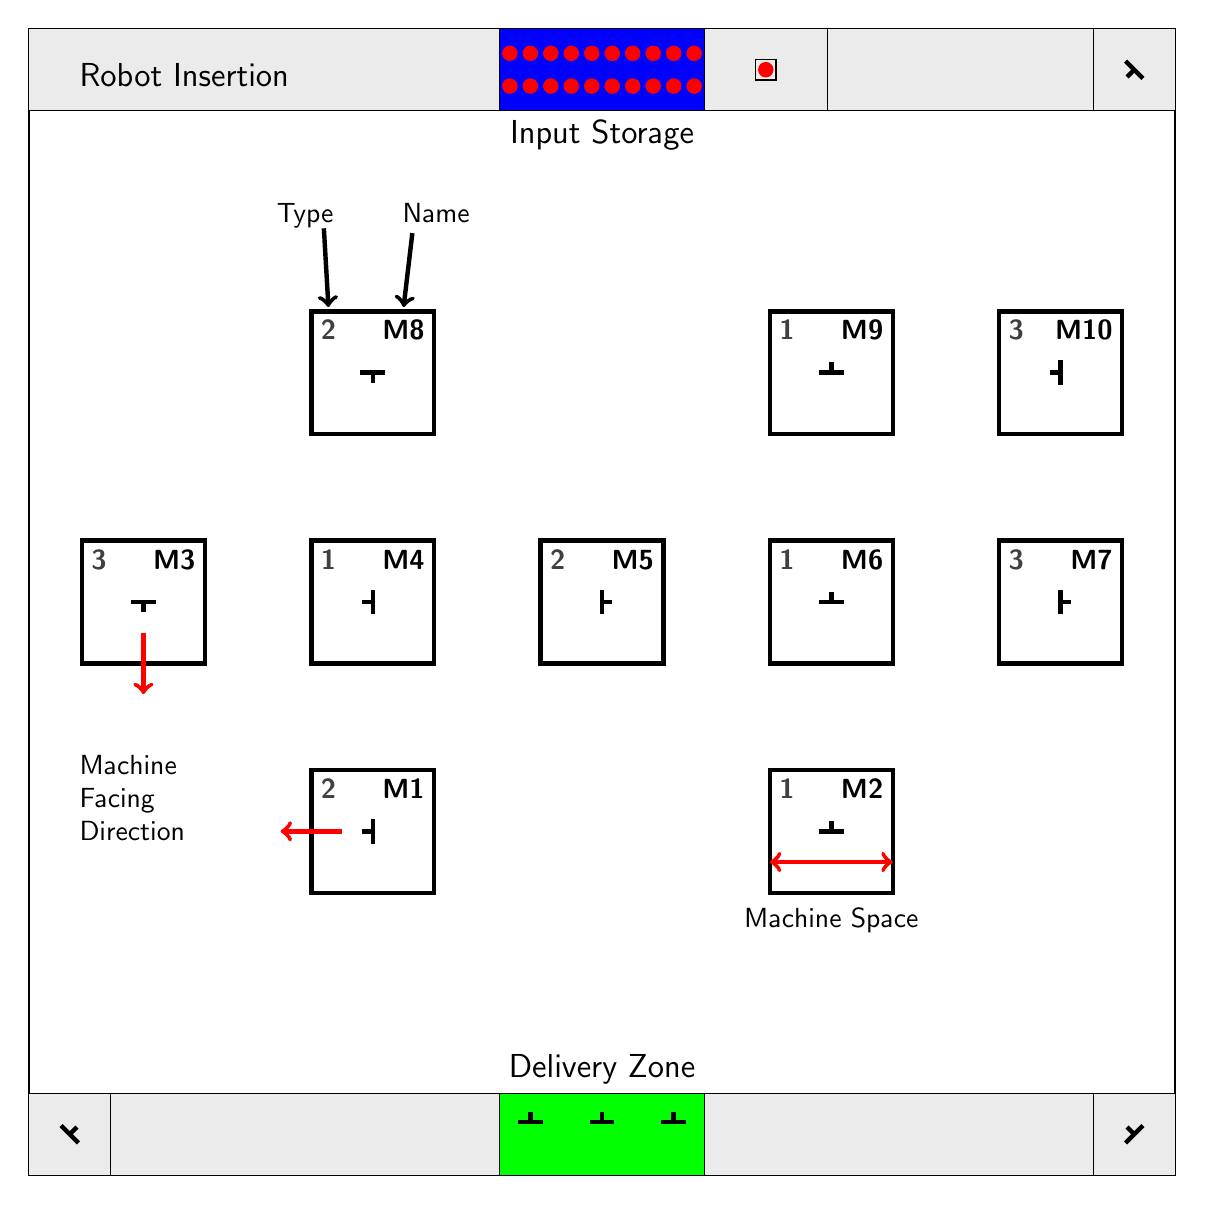
\begin{tikzpicture}[scale=2.6]
    % field outline
    \draw [thick] (0,0) rectangle (5.6,5.6);
    %\draw [fill=black!8] (0,0.4) rectangle (5.6,5.2);
    \draw [fill=black!8] (0,0) rectangle +(5.6,0.4);
    \draw [fill=black!8] (0,5.2) rectangle +(5.6,0.4);

    % margin areas
    \draw (0,0.4) -- (5.6,0.4);
    \draw (0,5.2) -- (5.6,5.2);
    \draw (0.4,0) -- +(0, 0.4);
    \draw (5.2,0) -- +(0, 0.4);
    \draw (5.2,5.2) -- +(0, 0.4);
    \draw (3.9,5.2) -- +(0, 0.4); % express good area vertical line
    \draw (2.3,0) [fill=green] rectangle +(1,0.4);
    \draw (2.3,5.2) [fill=blue] rectangle +(1,0.4);
    % express good slot
    \draw (3.55,5.35) rectangle +(0.1,0.1);
    \draw (3.6,5.4) [fill=red,draw=red] circle (0.035);

    \foreach \m/\t/\x/\y/\ori/\paintbox in
    % row 1, M1 M2
    { M1/2/1.68/1.68/180/1, M2/1/3.92/1.68/90/1,
    % row 2, M3 M4 M5
      M3/3/0.56/2.80/-90/1, M4/1/1.68/2.80/180/1, M5/2/2.80/2.80/0/1,
    % row 2, M6 M7
      M6/1/3.92/2.80/90/1, M7/3/5.04/2.80/0/1,
    % row 3, M8 M9 M10
      M8/2/1.68/3.92/-90/1, M9/1/3.92/3.92/90/1, M10/3/5.04/3.92/180/1,
    % recycling 1, recycling 2, test station
      R1/R/0.20/0.20/45/0, R2/R/5.40/5.40/-135/0, Test/T/5.40/0.20/135/0,
    % delivery stations
      D1/D/3.15/0.26/90/0, D2/D/2.80/0.26/90/0, D3/D/2.45/0.26/90/0
    }
    {
      \draw [ultra thick] (\x,\y) -- +($ (\ori-90:0.06)$);
      \draw [ultra thick] (\x,\y) -- +($ (\ori+90:0.06)$);
      \draw [ultra thick] (\x,\y) -- +(\ori:0.05);
      \if\paintbox1
        \draw [ultra thick] ($ (\x,\y) - (0.3,0.3) $) rectangle +(0.6,0.6);
        \draw [anchor=north east,inner sep=1pt] ($ (\x,\y) + (0.27,0.27) $)
          node (\m) {\selectfont\sffamily\textbf{\m}};
        \draw [anchor=north west,inner sep=1pt] ($ (\x,\y) + (-0.27,0.27) $)
          node (\m-\t) {\color{black!75}\selectfont\sffamily\textbf{\t}};
      \fi
    }

    \foreach \x in {1,2,...,10}
    {
      \draw ($ (2.25,5.48) + (\x*0.10,0) $) [fill=red,draw=red] circle (0.035);
      \draw ($ (2.25,5.32) + (\x*0.10,0) $) [fill=red,draw=red] circle (0.035);
    }


    \node [anchor=south west] at (0.2,5.27) {\large\sffamily Robot Insertion};
    \node [anchor=north] at (2.8,5.2) {\large\sffamily Input Storage};

    \draw [<->,red,thick,ultra thick] (3.62,1.53) -- +(0.6,0);
    \node [anchor=north] at (3.92,1.35) {\sffamily Machine Space};

    \node [anchor=south] at (2.8,0.4) {\large\sffamily Delivery Zone};

    \draw [->,red,ultra thick] (0.56,2.65) -- +(0,-0.3);
    \draw [->,red,ultra thick] (1.53,1.68) -- +(-0.3,0);
    \node [anchor=north west,text width=1cm] at (0.2,2.1)
    {\sffamily Machine\\Facing\\Direction};

    \node (name) [anchor=north,inner sep=0pt] at (1.99,4.75) {\sffamily Name};
    \node (type) [anchor=north,inner sep=0pt] at (1.35,4.75) {\sffamily Type};

    \draw [->,black,ultra thick]
    ($ (name.south west) + (0.05,-0.05) $) -- ($ (M8.north) + (0,0.05) $);
    \draw [->,black,ultra thick]
    ($ (type.south east) + (-0.05,0) $) -- ($ (M8-2.north) + (0,0.05) $);

  \end{tikzpicture}
  \caption{Competition Area}
  \label{fig:competition-area}
\end{figure}



\subsection{Coordinates of the Production Machines}
\label{sec:coordinates}

\begin{table}[h]
  \centering
  \begin{tabular}{l|r|r}
    \multicolumn{1}{l}{Number} & \multicolumn{1}{l}{$X~[m]$} & \multicolumn{1}{l}{$Y~[m]$}\\ \hline
    Machine 1 & 1.68 & 1.68 \\
    Machine 2 & 3.92 & 1.68 \\
    Machine 3 & 0.56 & 2.80 \\
    Machine 4 & 1.68 & 2.80 \\
    Machine 5 & 2.80 & 2.80 \\
    Machine 6 & 3.92 & 2.80 \\
    Machine 7 & 5.04 & 2.80 \\
    Machine 8 & 1.68 & 3.92 \\
    Machine 9 & 3.92 & 3.92 \\
    Machine 10 & 5.04 & 3.92 \\
    Recycling unit 1 & 0.20 & 0.20 \\
    Recycling unit 2 & 5.40 & 5.40 \\
    Test station &	5.40  &0.20 \\
    Express good insertion point / slot & 	3.60 & 	5.35 \\
    Delivery slot 1 & 	3.15 & 0.26 \\
    Delivery slot 2 &	2.80 & 0.26 \\ 
    Delivery slot 3 &	2.45 & 0.26 \\\hline
  \end{tabular}

  \caption{Coordinates of production machines}
  \label{tab:coordinates}
\end{table}

\subsection{The Pallet Carrier Puck}
The data carrying RFID tag is mounted to a hockey puck. The tournament
puck features a diameter of 7.5cm.

\begin{figure}[h!]
  \centering
  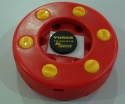
\includegraphics[height=3cm]{125px-Puck}
  \caption{Puck}
  \label{fig:puck}
\end{figure}

\subsection{Machines}
\label{sec:machines}

\subsubsection{General Information}

\begin{figure}[h]
  \centering
  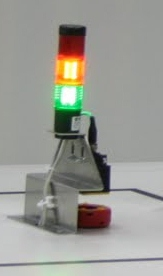
\includegraphics[height=6cm]{Machine}
  \caption{Machine}
  \label{fig:machine}
\end{figure}

All machines are identical devices consisting of 
\begin{itemize}
\item one plate housing the RFID read/write device and
\item one signal unit according to the figure above.
\end{itemize}

They share the same design and the same RFID device, with the overall
size of 280 mm height, 160 mm of width and 100 mm of depth, see the
engineering reference for further details. The default operating mode
of all machines implies that only the green LED is turned on. This
signals the machine being ready for input. The reading and writing
process generally is a delicate process. To avoid corruption of the
data carrier, it should not leave the working range of the RFID device
once the processing or consuming is started. To enable the production
process it is necessary to transport the pallet carrier accurately to
the RFID device. A consumed pallet carrier has to stay within the
machine space borders(no part of the puck being outside the mark-up)
until the production cycle of that very machine has been
completed. Production resulting from violating this requirement is
considered junk and will not be rewarded. The machine always processes
the required pallet carrier delivered last, all prior components will
be consumed. All machines will start processing the data carrier as
soon as they enter the diameter named below and change their operating
mode according to the tables provided.


\subsubsection{Production Machines}
After processing the current data carrier: Yellow LED turned on The
machine has finished processing the current data carrier and is
waiting for the next subassembly. Green LED turned on The machine has
finished the work order and is ready to receive the next batch of
carriers. In order to complete the machines' work order the input
materials have to be delivered one-by-one into the RFID device's
action range. Multiple data carriers in range of the device will
result in erroneous behavior of the device. Consumption of materials,
like \s0 used in the production of \s2, will take 2 seconds. Unloading
the machine can be done immediately after the operating mode changes
away from processing. As long as the machines are used properly, they
will not produce any junk.

\begin{table}[h]
  \centering
  \begin{tabularx}{\linewidth}{p{0.35\linewidth}|X}
    \multicolumn{1}{l}{Optical Feedback} &
    \multicolumn{1}{l}{Operating mode} \\ \hline
    All LEDs turned off &  	The machine is physically offline, caused by a real error which should not happen during the competition. \\
    Red LED turned on &  	The machine is out of order \\
    Green LED turned on &  	The machine is idle and ready.\\
    Green and yellow LED turned on &  	The machine is processing or consuming the current data carrier. \\
    Yellow LED flashing(at 2 Hz) & The machine detects wrong material.
    This can be caused by data carriers that are already consumed,
    subassemblies that do not fit to this machine type's work order or
    corrupted data carriers. \\\hline
  \end{tabularx}


\bigskip
%\begin{rulechange}
  \begin{tabularx}{\linewidth}{l|X|X|X|l}
    \multicolumn{1}{l}{ Type} & \multicolumn{1}{l}{Distribution} & \multicolumn{1}{l}{Input} & \multicolumn{1}{l}{Output} & \multicolumn{1}{l}{(Final)processing time[s]}\\\hline
    \m1 & 4 times & \s0 (Raw-material) & \s1 & $WT_1 = 3 \mbox{ to } 8~\mathrm{sec}$\\
    \m2 & 3 times & \s0; \s1 \s2; & \s2; one consumed container & $WT_2 = 15 \mbox{ to } 25~\mathrm{sec}$\\
    \m3 & 1 times &	\s0;\s1;\s2 & \p1; two consumed containers &$WT_3 = 40 \mbox{ to } 60~\mathrm{sec}$\\
    \m4 & 1 times &\s0;\s1;\s2 & \p2; two consumed containers &$WT_4 = 40\mbox{ to } 60~\mathrm{sec}$\\
    \m5 & 1 times &	\s0; & \p3; one consumed container &$WT_5 =40\mbox{ to } 60~\mathrm{sec}$
  \end{tabularx}
%\end{rulechange}
  \caption{Production Machines}
  \label{tab:production-machines}
  
\end{table}



The distribution describes how many machines of the respective types
will be randomly placed resulting in a the total of 10 court machines.



\subsubsection{Recycling Unit (former market place)}
The recycling unit processes all supplied loading carriers back to
raw-material (\s0) within 2 seconds.

\begin{table}[h]
  \centering
  \begin{tabularx}{\linewidth}{p{0.35\linewidth}|X}
    \multicolumn{1}{l}{Optical Feedback} &\multicolumn{1}{l}{Operating
      mode}\\\hline
    All LEDs turned off & 	The machine is physically offline, caused by a real error which should not happen during the competition.\\
    Red LED turned on & 	The machine is out of order\\
    Green LED turned on & 	The machine is idle and ready.\\
    Green and yellow LED turned on & The machine is processing the
    current data carrier.\\\hline
  \end{tabularx}
  \caption{Recycling Unit}
  \label{tab:recycling-unit}
\end{table}



\subsubsection{Reading device}
The reading and visualizing the data carriers content happens almost
instantly after delivering the pallet carrier to the action range of
the device.

\begin{table}[h]
  \centering
  \begin{tabularx}{\linewidth}{p{0.35\linewidth}|X}
    \multicolumn{1}{l}{Optical Feedback} &\multicolumn{1}{l}{Stored
      data on the data carrier}\\\hline
    Green LED turned on &	The station is ready to read the next data carrier.\\
    All LEDs turned off &	Consumed pallet carrier.\\
    Yellow LED turned on &	Raw-material (\s0) \\
    Red and yellow LEDs turned on & 	Subassembly 1 (\s1)\\
    Red LED turned on &	Subassembly 2 (\s2)\\
    All LEDs turned on & The final product (\p{})\\\hline
  \end{tabularx}
  \caption{Reading Device}
  \label{tab:reading-device}
\end{table}

\subsubsection{Delivery Gates} \begin{table}[h]
  \centering
  \begin{tabularx}{\linewidth}{p{0.35\linewidth}|X}
    \multicolumn{1}{l}{Optical Feedback} &\multicolumn{1}{l}{Stored
      data on the data carrier}\\\hline
    Red LED turned on & This delivery gate is inactive.\\
    Red and green LED turned on & This gate is active, namely the designated gate.\\
    \hline
  \end{tabularx}
  \caption{Delivery Gates}
  \label{tab:delivery-gates}
\end{table}

As soon as a pallet carrier is successfully delivered to the active
gate, it will show the state of the data carrier as described above.
This state will only long for some seconds and only for scoring
reasons. There will be only one active gate at a time.


%%%%%%%%%%%%%%%%%%%%%%%%%%%%%%%%%%%%%%%%%%%%%%%%%%%%%%%%%%%%%%%%%%%%%%%%%%%%%
%%%

\section{The Robotino System}

All participants have to design their competition Robotinos within
the following specifications:

Any kind of sensors can be changed or added to the Robotino platform.
However, it is not possible to implement sensors that require
modifications outside the Robotino area (e.g. Northstar, indoor GPS).
It is furthermore strictly forbidden to implement any kind of RFID
device into the Robotino. There must be no changes to the controller
or mechanical system. The pushing device is defined as a passive,
non-mechanical load handling attachment. The robots peripherals must
neither exceed the maximum total height of 0.7 m nor the 0.4 m
diameter of the body cylinder. The only exception to this is the one
default mounted pushing device per robot. The pushing device can be
modified; it however must not exceed the following outside dimensions:
0.25 m x 0.15 m x 0.05 m.

%\begin{rulechange}
  It is allowed to install additional computing power on the
  \Robotino. This may either be in form of a notebook/laptop device or
  any other computing device that suits the size requirement of the
  \Robotino{} competition system. Furthermore, it is allowed to
  communicate with an additional computing device off-field. This
  device may be used for team coordination and/or other
  purposes. However, communication among the robots and the off-field
  device is not granted during the competition.
%\end{rulechange}

For a detailed technical description, refer to the Engineering
Specifications chapter 1.1 

\section{Communication}
Robots have to operate autonomously, that is without any human
interference during the game. Communication among robots and to
off-board computing units is allowed only using wifi
(cf.~\refsec{sec:wifi-regulations}. Communication is not guaranteed
and maybe unavailable during parts of the game. Interruptions must be
expected and is no reason to pause or abort a game, even if they
endure for long periods of the game.

\subsection{Bandwidth Allocation}
\label{sec:bandwidth}
No minimum bandwidth is guaranteed. The amount of communicated data
over the wifi connection shall not exceed 2\,MBit/sec. Even though the
lower layers could provide for more bandwidth, the overall available
frequency spectrum and wifi channels have to be shared, not only
within our own league. Generally, a conservative use of bandwidth
resources is advised. Should a frequently or endured exceedance
exceedance of the bandwidth limit become known, or if the overall
bandwidth limit must be reduced due to out circumstances, the TC can
monitor the network traffic and demand reduction in communicated
data as necessary.

\subsection{Referee Box}
\label{sec:refbox}
The referee box (refbox) is a software system that runs on a system
provided by the Organization Committee. It controls the overall game,
monitors feedback from team robot, and awards points. It is instructed
by a assisting human referee.

To be completed:
\begin{itemize}
\item protobuf
\item Message type overview
\item Single point of robot instruction
\end{itemize}

The protocol and technical specifications are described in detail in
the RoboCup Logistics League Referee Box documentation.

\subsection{Inter-Robot Communication}
\label{sec:inter-robot-comm}

\subsection{Communication Eavesdropping and Interference}
\label{sec:comm-tampering}
% This might sound harsh, but it's based on lessons learned in
% numerous years of RoboCup, you wouldn't believe what some teams will
% do... :-/
Communication of another team may neither be eavesdropped on nor be
interfered with. Teams not currently active shall disconnect from the
field access points.

Monitoring of bandwidth used or of possible misbehavior may only be
performed by members of the TC.
% can add this, need to be clear that this must be done using a team
% leader majority vote and not just any team leader
% or by a person appointed by the team leaders.
Any indication of misbehavior will be discussed by the team leader
convention and may result in penalties or disqualification from the
tournament.


%Each robot has to operate autonomously. The communication between the
%robot and the device responsible for the Start/Stop command, as well
%as all communication amongst the robots has to be realized using the
%Wi-Fi connection. The program controlling the robot has to be executed
%locally by the robot itself. % It is strictly forbidden to use any kind
%% of external server acting as command point.
%\begin{rulechange}
%  The robots will receive their commands from the Referee-Box as
%  specified in the referee box protocol. Further, communication to one
%  dedicated off-board computing device is allowed. However, wifi
%  communication should not taken for granted during competition by the
%  participating teams. 
%\end{rulechange}
%The robots are allowed to share information with other devices, but
%must receive nothing else but the start, pause and stop command
%from units other than the 2 fellow robots. This specifically excludes:
%Usage of processed image data created outside of the robots A central
%communication that requires a device other than the three Robotinos A
%permanently established connection between the command device and the
%Robotinos.

\subsection{Wifi regulations}
\label{sec:wifi-regulations}
In order to provide the optimal possible solution for wireless
communication during the event, all teams are required to use the 5
GHz Wi-Fi equipment. They are furthermore required to connect their
Robotinos Wi-Fi unit to the access point provided. All teams can also
relay on Wi-Fi clients supplied by Festo but are not required to. A
detailed description concerning the infrastructure can be found in
chapter 1.8 of the Engineering Specifications.

% Please refer to Sect.~\ref{sec:radio-interference} for further details.

%%%%%%%%%%%%%%%%%%%%%%%%%%%%%%%%%%%%%%%%%%%%%%%%%%%%%%%%%%%%%%%%%%%%%%%%%%%%%
%%%

\section{Tournament}
\subsection{Setup}

A match is defined by two contesting teams competing at two separated
identical competition areas. Each match lasts 15 minutes with 5
minutes of setup time and a 2 minute Exploration Phase. All settings, including
the EGC and random events, will be the exact same for both parties of a match.

\subsection{Team setup}
\label{sec:team-setup}
No team member is allowed to enter the competition area prior to or
during a match. The robots can be set up within the robot insertion
area as long as they are outside the factory area and have not been
elevated into their autonomous state. During a match the manipulation
is limited to adjustments on sensors, checking cable connections and
the boot or shut down procedure. A team can ask the referee to shut
down the robot. If this motion has been forwarded within the first 15
seconds of the very robots movement and without this robot scoring
points, the referee will move it to a point of insertion of the team's
choice, once. Otherwise or on second occasion the robot will be
removed from the competition area. Resetting or removing a robot will
not cause an interruption of the game. The referee will only interrupt
the game if there is no other way to reset the robot without
interfering with the other ongoing processes. Once removed from the
competition area the robot cannot be reinserted during the same match.
A team can also decide to remove their robot from the competition area
at any time of the match.

\subsection{Setup environment}
\subsubsection{Machine Initialization}

The physical distribution of the production machines is fixed. Their
alignment will be randomized during the event setup but will stay that
way through the whole event. The machine type of each production
machine will be randomized prior to each match. The processing time of
each machine type will be determined in the same way, so the waiting
time during a match will be static for each machine of the three
machine types (e.g. all M1 could have 7 seconds processing time). The
active delivery gate will also be randomized prior to each match but
during a match the active gate can switch.


\subsubsection{Radio Interference}
\label{sec:radio-interference}
The referee will induce a connection breakdown between the command
unit and the Robotinos at certain points of a match. This will not
affect the Wi-Fi connection between the Robotinos and will neither
happen during the first minute of a match. Once switched off, the link
between LAN and Wi-Fi will stay severed for 100 seconds. The link will
be reactivated swiftly in case of emergency to interrupt the autonomy
of the process.


\subsection{Exploration Phase}
%\begin{rulechange}
Before the actual game starts, the machines will indicate their types with the
signal lights for two minutes. The robots are to roam the environment and
announce detected signals to the Referee-Box. Each properly reported signal
scores two points, each signal reported wrongly will give -1 points penalty.
A minimum of zero points will be accounted for this exploration phase.
Production or moving Pucks is not allowed during the exploration phase.
%\end{rulechange}

\subsection{Match startup}

All matches will start at the exact time scheduled by the organization
team. From this point on, the teams involved are allowed to start
their robots to work autonomously. This can be done by one click per
robot on any kind of interface. 

%\begin{rulechange}
As a start signal the Referee-Box will initially announce the true assignment of
all machines to the robots.
%\end{rulechange}

\subsection{During a match}

The referee can interrupt the match at any time. Then, both teams have
5 seconds to stop all robot movement. The match time will be paused
during the interruption. A team can decide to stop the autonomy
process of each robot individually at any time of the match. Doing so
has to be announced notably in order to inform the referee, as this is
considered a shut down request according to
\ref{sec:team-setup}. Robots that do not stop within the time limit
will be treated in the same way.

\subsubsection{Out-of-order}

The downtime generator will take down a maximum of two machines out of
the pool containing production machines and recycling units. It will
do so at random points of time. There will be 6 to 8 of such triggered
events during a match. The machines affected will remain out of order
for 60 to 120 seconds. Every machine can only be forced out of order
once per match. If the machine turns offline during processing or
consumption of mounted a pallet carrier, it will afterwards resume the
process.

\subsubsection{Production Plan}

%\begin{rulechange}
The Referee-Box will announce a production plan for three different phases of
the match. The production plan specifies how many items of different product
variant have to be produced in the current production phase. Only products which
are covered by the production plan score. In 2013 each of the three phases will
last 5 minutes. The first phase will start with the match startup.  The second
phase will start at minute 5, the third at minute 10.

%\end{rulechange} 

\begin{table}[h]
  \centering
  \begin{tabularx}{\linewidth}{p{0.35\linewidth}|X}
    \multicolumn{1}{l}{Product Variant} &\multicolumn{1}{l}{Demanded number of items } \\
    \hline 
    Product Variant \p1 &	$N_1 = 1 \mbox{ to } 10$ items \\
    Product Variant \p2 &	$N_2 = 1 \mbox{ to } 10$ items \\
    Product Variant \p3 &	$N_3 = 1 \mbox{ to } 10$ items \\
	\hline
  \end{tabularx}
  \caption{Production plan}
  \label{tab:production-plan}
\end{table}

\subsubsection{Express good challenge}

%\begin{rulechange}
The challenge will be induced by the Referee-Box sending an Expres-Good-Message
to the robots. The Message specifies the demanded product variant, a time-window
and the delivery gate. As a first step the Express-Good-Challenge of 2013 will
only demand product variant \p3. Furthermore, in 2013 the challenge has to be
completed within a time-window of 120 seconds and the express good has to be
delivered to the active delivery gate.
%\end{rulechange}

\subsection{Mode}
\subsubsection{Tournament specifications}

The tournament features two stages with the first stage being done in
league form with several sequels orientating at the number of
participants and a second stage with playoffs featuring the top 4
teams.

Each match will be resulted with the score of each team. The winning
team will be awarded 2 major points. In case of a draw both teams will
be awarded with 1 major point. In case both teams scored zero points,
no major points will be awarded.

In case of a draw within the playoffs, the game time will be extended
by 5 minutes unless both teams scored zero points.

If this extension leads to a draw too the overall regular points of
the teams will determine the match winner. If the overall points are
equal too, a direct comparison between the teams in question will
decide. If this fails to resolve the situation, the teams will
approach a coin toss to determine the winner.

The detailed seeding will be created at the event. Although the idea
is to allow each participant to challenge each other team the league
can be adjusted to meet time requirements.


\subsubsection{Tournament challenge}
Proceeding to the playoffs will result in the following changes to the EGC setup:
% \begin{table}[h]
%   \centering
%   \begin{tabularx}{\linewidth}{l|X}
%     \multicolumn{1}{l}{Phase} &\multicolumn{1}{l}{Remark}\\\hline
%     \multirow{7}{*}{League phase} & 
%     \begin{itemize}\itemsep-3pt
%     \item The active delivery gate will not switch during a match.
%       % 
%     \item There will be 3 express good challenges.
%       % 
%     \item     No challenge will be initialised during the first or within the last two match minutes.
%     \end{itemize} \\
%     \multirow{9}{*}{Playoffs} &
%     \begin{itemize}\itemsep-3pt
%     \item The active delivery gate will swap twice - after minutes 7
%       and 11. A delivery made to the old active gate will be still
%       valid for the next 10 seconds.
%       % 
%     \item There will be 4 express good challenges. 
%       % 
%     \item No challenge will be initialised during the first or within
%       the last two match minutes.
%     \end{itemize}\\\hline
%   \end{tabularx} 
%   \caption{Tournament Phases}
%   \label{tab:phases}
% \end{table}

\paragraph{League phase}~\\
\begin{itemize}
\item The active delivery gate will not switch during a match.
\item There will be 3 express good challenges.
\item No challenge will be initialised during the first or within the
  last two match minutes.
\end{itemize} 

\paragraph{Playoffs}~\\
\begin{itemize}
\item The active delivery gate will swap twice - after minutes 7
  and 11. A delivery made to the old active gate will be still
  valid for the next 10 seconds.
\item There will be 4 express good challenges. 
\item No challenge will be initialised during the first or within
  the last two match minutes.
\end{itemize}
     

In both cases, delivered or timed out pallet carriers will be removed
from the game by the administration and therefore cannot be recycled.

\subsubsection{Task fulfilment?}

The following table provides the itemized clearance of all task
related processes.
\begin{table}[h]
  \centering
\begin{tabularx}{\linewidth}{p{6em}|X|p{4em}}
  \multicolumn{1}{l}{Subtask } &\multicolumn{1}{l}{Main challenge} &
  \multicolumn{1}{l}{Scoring [Point]}\\\hline
  Produce \s2 & Finish the work order of a machine type 2 & $+4$\\
  Produce \p  & Finish the work order of a machine type 3 & $+12$ \\
  Deliver & Deliver the final product to the designated loading zone & $+5$\\
  Recycle & Clean up a polluted machine (\m2 or \m3) by recycling all
  of the 3 consumed loading carriers. Partial recycling(\m3) will not
  be rewarded.&
  \multirow{3}{*}{$\begin{array}{l}+3 - \m2\\
      +6 - \m3\end{array}$}\\
  Sum &Total points a team will receive for a produced and correctly
  delivered final product with its consumed loading carrier
  recycled. & $30$\\\hline
  \end{tabularx}  

\bigskip
\begin{tabularx}{\linewidth}{p{6em}|X|p{4em}}
    \multicolumn{1}{l}{Subtask } &\multicolumn{1}{l}{EGC - Expressgood Challenge} &
    \multicolumn{1}{l}{Scoring [Point]}\\\hline
    Finish the EG &	Deliver the EG to a machine of type 1 and process the express good in time if the machine type was identified by an earlier production process. &	+5\\
    Deliver the EG & Deliver the processed express good to the active
    delivery gate in time. &  +10\\
    Sum &  In time delivery of a correct
    express good. & 15\\\hline
  \end{tabularx}  

  \caption{Scoring Scheme}
\end{table}



\subsection{Penalties}

This catalogue represents the decision basis of the referee without
being exhaustive or binding.

\begin{table}[h!]
  \centering
  \begin{tabularx}{\linewidth}{l|X}
  \multicolumn{1}{l}{Issue} &\multicolumn{1}{l}{Sanction}\\\hline
  Premature movement & No robot is allowed to move until the referee
  announced the start of the match The faulty robot will be grounded
  for
  2 minutes\\[1ex]
%
  Damaging factory equipment & Theoretical damage to the real
  factory equipment as a result of collisions and negligent actions.
  The team will be punished with a score reduction. The total score
  cannot  drop below zero.\\[1ex]
%
  Not showing up & A team not showing up at all. The team will be
  removed from the tournament unless the team leader can provide a
  sincere explanation\\[1ex]
%
  Breaking a minor rule & A rule infringement with none or little
  impact on the team performance The team will receive a warning or a
  small  score reduction\\[1ex]
%
  Breaking a major rule & A rule infringement with considerable impact
  on the team performance or competition mechanics. The referee will
  decide upon calling a team vote or imposing an adequate punishment.\\[1ex]
%
  Arguing with the referee & There will be no discussions during a
  match. Each team can make a motion to protest a certain match and
  its result which will be dealt with after the match. There will be a
  warning. Continued disregard will result in a time punishment to the
  team's current or next match.\\[1ex]
%
  Disregarding rules of conduct & Following the rules of conduct
  should be self-explanatory Upon disregard, the referee will impose
  sanctions ranged from time punishments to the team's complete
  removal from the tournament.\\\hline
  \end{tabularx}  
  \caption{Infringements}
  \label{tab:infringements}
\end{table}



%\begin{rulechange}
  \subsection{Technical Challenge}
  
  Within the league, the technical advances should be documented from
  year to year. Therefore, the Technical Challenge is introduced.
  Each participating team should prepare for participating in any
  number the following tasks:


  \paragraph{Collision avoidance.~}
  The robot is to show that it avoids other obstacles and robots.
  Therefore the robot must drive from input storage to the delivery zone.
  However, the paths between the input storage and the delivery zone will
  be blocked randomly by static obstacles and the robot must not touch any
  of the obstacles. For touching an obstacle, the team receives a penalty.
  The fastest team with the fewest penalty points to reach the delivery
  zone wins this challenge. All other teams are ranked according to
  how fast they were and how many penalties they conceived.
  
  \paragraph{Whac-a-Mole.~}
  A single robot is placed somewhere on the field. It has to detect
  the single shining signal unit on the play field. As soon as it puts
  a puck underneath it, the signal unit is switched off and another
  random signal unit is switched on. The goal of the challenge is to
  switch as many signal units as possible within a given time
  frame. Teams are ranked according to the number of turned-off
  signals.
  
  \paragraph{Free challenge.~}
  Each team will be given 5 minutes to showcase their robot team, e.g.
  show some new robotics developments. The teamleaders of
  non-presenting team will judge the performance and rate it with
  points between 0--10.  The team with the most points will win this
  challenge. The other teams are ranked in decreasing point order.


  The technical challenge is conducted in the following way: The
  teamleader of each participating team agree on a date and time
  during the tournament for the Technical Challenge in their first
  Teamleader Meeting. Each team can register for any of the
  challenges. All teamleaders have to be present at the time of the
  challenge to judge the other teams. The OC is responsible to conduct
  the Technical Challenge and can appoint teamleaders to support in
  conducting the challenges. Each challenge will have a separate
  ranking. In each ranking, the team on the last rank will receive 0
  points, the last-but-one ranked team will receive 1 point etc. The
  points for each ranking will be added and the team with the most
  points accrued over all challenges will be awarded with the
  LLSF Technical Challenge Award.

%\end{rulechange}

%%%%%%%%%%%%%%%%%%%%%%%%%%%%%%%%%%%%%%%%%%%%%%%%%%%%%%%%%%%%%%%%%%%%%%%%%%%%%
%%%

\section{Development / Vision}

This section is meant to enable discussions and support investment
decisions for future soft- and hardware acquisitions.

\subsection{Short term ideas}

These are ideas that could still be incorporated into the rulebook of
Istanbul 2011. 

\subsubsection{Scripted, dynamic obstacles}

On the way to fully dynamic obstacles this iteration implies a fully
scripted administration controlled Robotino that follows implicit
movement rules that are known to all participants.

\subsection{Midterm planning}
Additions and alterations for future iterations of this competition


\subsubsection{Various Production programs}
A part from the three-staged production process, various goods with
different work orders and specifications (e.g. top speed, delivery
strategies...) could be part of the challenge. This addition seems to
be heavily dependent on Sect.~\ref{sec:supp-flow}.

\subsubsection{Various order strategies}
A delivery could consist of more than one final product, it could be
required to deliver a batch of products, maybe within a certain time
span, to complete the loading and receive extra points. Also, the
different delivery gates could obtain a predefined shipping list, for
example gate 1 requiring 2 Products, 2 M2 and 1 M1, maybe in the
correct order to enable FIFO, LIFO or other delivery strategies.

\subsubsection{Simulation league}

Since there is only the annually world championship and maybe a
regional preregistration, a simulation platform could be provided,
where the software framework of teams can be used to compete with
other teams. Additionally a branch of simulation could be created that
focuses on the simulation of many AGV and a huge production area in
order to compete on scalability.

\subsubsection{Introducing a supportive flow of information}
\label{sec:supp-flow}

As the current task only deals with the material stream, it is heavily
limited to a simple static task. In order to enable a flow of
information that transports complex orders, a combined effort should
focus on implementing a data interface that can be used by all teams
today and in the future. As this would be a giant leap towards the
industrial application, a general discussion and a lot of effort has
to be invested into this issue.


\subsection{Long term Vision}
Ideas, dreams and ideology that inspire the future development.

\subsubsection{Complex production machines}
As there are more ways to interact with a machine than mounting and
dismounting a loading carrier, it is possible to develop new machine
types that look different and are completely different to handle.

\subsubsection{Collaborative Production}
Teams could be required to cooperate with another team to enable a
combined supply chain. 

\subsubsection{Opponent controlled dynamic obstacles}
No scripted obstacle can truly represent challenges of the industrial
application. In the long run, an opposing team has to be reinserted
that is allowed and requested to anticipate the logistic processes in
real time in order to create worst case scenarios for the teams.

\subsubsection{Interfacing ERP / SCM}
The interface used to present orders could be back ended with software
from real business applications like ERP, PPS, WHM and SCM.

\subsubsection{JIS / JIT implementation}
With complex production processes and several other achievements and
upgrades it could be useful to implement JIS and JIT tasks and
procedures into the LL, requiring delivery strategies like LIFO, FIFO
and certain time windows.



 
\end{document}
